\section{Introduction} \label{sec:introduction}

% What are containers and why they are becoming popular: pointing out portability and resource efficiency.

Containerization is a lightweight and efficient virtualization technology that 
wraps a piece of software in a complete filesystem cell which is called as a 
{\em container}. 
One container contains everything needed to run -- code, runtime, system tools, s
system libraries -- and guarantees that the software will always run the same on 
top of a proper host OS kernel. Containerization is rapidly
becoming popular for deploying applications in data centers, 
due to its good agility 
and portability of code deployment and high efficiency of resource sharing, 
compared with virtual machines (VMs)~\cite{?}. In essence, one container is
one process with its own namespace and resource group isolated with other's,
and such isolation eliminates the dependencies and interferences in running 
environments of different processes on the same host.

% Currently, container networking is only using IP networks. It has large overhead in resource efficiency and performance.

Nevertheless, the isolation among containers can also lead severe efficiency
problems in networking. TCP/IP is the de facto container networking solution. 
To support TCP/IP, container runtime systems, such as Docker~\cite{?} and
Kubernetes~\cite{?}, connect containers with virtual networks and route IP 
packets among containers with software. This solution offers portable 
connectivity and strong isolation to containers, but TCP/IP's poor performance
and large overhead make it not suitable for all applications in data centers.
First of all, it is difficult and expensive to achieve high throughput with TCP/
IP. TCP/IP inherently split data into packets and each packet can generate 
numerous system calls, interrupts, task switches and data coping, etc., which 
cost tremendous CPU cycles. \S\ref{sec:motivation} shows that CPU will quickly 
becomes the bottleneck which limits the throughput of TCP/IP. Additionally, 
traversing the whole TCP/IP and software network stack significantly stretches 
the network latency which quickly becoming the limiting factor in applications
like in-memory cache, key-value stores and machine learning~\cite{?}.

% Other options for networking.
Apart from TCP/IP, there are still several options for container networking,
while they all have their own pros and cons and have not been used by containers.
For instance, containers are essentially processes on the host OS, and they can 
communicate via IPC channels, like shared-memory which can bypass the whole OS 
stack. This solution can achieve
excellent network performance in both throughput and latency as shown in \S\ref{s
ec:motivatoin}, but requires the containers are co-located in the same host and 
trust each other. Another promising option is remote direct access memory (RDMA) network stack. It does not only have good network performance and low CPU overhead but also good portability regardless the locations of containers. 
However, it needs special hardware supports, and we also found that it is not efficient for containers in the same host to use RDMA
(see \S~\ref{sec:motivation}). 

Since different applications have specific concerns on the performance, 
isolation, portability and overhead, there is no
one-size-fit-all container networking solution. To make the communications among
containers more efficient, a proper network solution should be adopted according
to application requirements, container locations and hardware capabilities.
For example, if one micro-service application has a group of containers trusting each other, and it cares most about network performance, it had better use
shared memory to connect the containers on the same host, and RDMA on different hosts when the hardware is capable. 

On the flip side, switching among multiple network solutions can potentially 
make the application code extremely complicated. This is because
containers must use different programming interfaces for different
network solutions. For instance, TCP/IP requires socket API, and POSIX and Verbs
are common API for shared-memory and RDMA respectively. 
It will be favorable if the network solution selection can be transparent to the application code.

\begin{figure*}[!ht]
     \centering 
     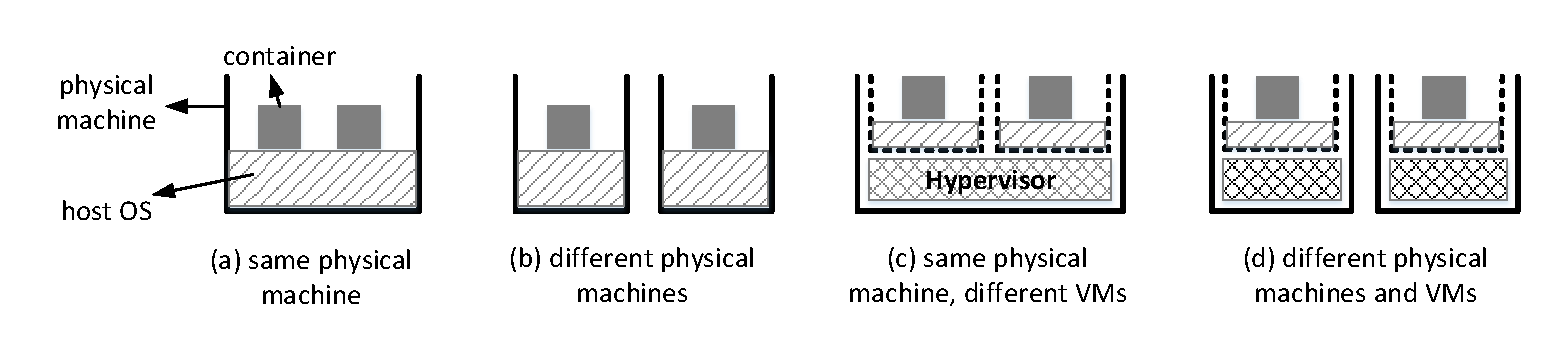
\includegraphics[width=6.7in]{figures/deployment-cases} 
    \caption{\label{fig:deploy-cases} Representitive running environments of containers.} 
\end{figure*} 

% What we do
In this paper we ask a simple question: {\em how can containers always have the best network properties for them with a uniform API?}
To answer this questions, we present~\sysname, a new abstraction layer for container networking to achieve close-to-optimal network properties. 
On one hand, \sysname has a network orchestrator integrated in container runtime systems that decides which network solution to use on-the-fly according to factors as the containers' locations, software stack and hardware capability. One the other hand, \sysname provides a simple and uniform programming interface for container communications.   

% What are the challenges
We are facing three main challenges in the design of~\sysname. First of all, 
how to design the uniform network API. One option is to define a brand new API 
set, but it is difficult not only because the complexity of designing a complete
and widely accepted API but also the training overhead to programmers.
Therefore, we decide to use an existing and mature API. Among the numerous candidates, e.g. socket, RDMA verbs, MPI, etc., we choose RDMA Verbs for two
reasons. First, RDMA Verbs has been widely accepted as an industrial standards and many applications desiring high network performance have already been using it~\cite{?}; Second, as a general communication interface, RDMA verbs can easily serve as a base layer supporting messaging (e.g. UDP,
MPI), streaming (e.g. TCP) and memory sharing (e.g. shared-memory, RDMA) on top of it.

Next, \harry{how to compatible with legacy verbs code.}

Finally, \harry{we should talk about the system challenges, but I do not know what exactly they are currently}.